\documentclass[a4paper]{article}

\usepackage[english]{babel}
\usepackage[utf8]{inputenc}
\usepackage{fullpage}
\usepackage{amsmath}
\usepackage{graphicx}
\usepackage[colorinlistoftodos]{todonotes}
%\usepackage{hyperref}
\usepackage{amssymb}
\usepackage{subfigure}
\usepackage{url}
\usepackage[pagebackref=true,colorlinks,linkcolor=red,citecolor=green,breaklinks=true,bookmarks=false]{hyperref}
\usepackage{outline} 
\usepackage{pmgraph} \usepackage[normalem]{ulem}
\usepackage{graphicx} \usepackage{verbatim}
\usepackage{indentfirst}
\setlength{\parindent}{2em}
% \usepackage{minted} % need `-shell-escape' argument for local compile

\title{
    \vspace*{1in}
    
\includegraphics[width=2.75in]{figures/zhenglab-logo} \\
    \vspace*{1.2in}
    \textbf{\huge Weekly Work Report}
    \vspace{0.2in}
}

\author{Hongzhi Liu \\
    \vspace*{0.5in} \\
    \textbf{VISION@OUC} \\
    \vspace*{1in}
}

\date{\today}


\begin{document}
\par
\maketitle
\setcounter{page}{0}
\thispagestyle{empty}
\newpage


\section{Research problem}

During this period of week, I spend time studying deep learning courses and working about Faster R-CNN algorithm for URPC2018. Our team have difficulty in changing competition data sets into VOC format and training a model for contest.

\section{Research approach}

For deep learning, I watch videos and write down the issues which I think are much important for further research. As for URPC2018, I continue to learn about Faster R-CNN algorithm \cite{Ren2015Faster} and try to train the First model with VOC2007. Besides, our team have prepared competition data sets for training contest model. I will list details about weekly work in Tab.~\ref{t2} below.
\begin{table}[hb]
	\centering
	\caption{Weekly work progress.}
	\begin{tabular}{c|p{10cm}}
		\hline 
		 & Finish training the first VOC2007 model and outcome is good.    \\
		
		 URPC2018 & Finish changing the txt truth table into xml files which are used for training contest model.\\
		 
		 & Finish putting confusing contest data sets in VOC2007 order from 000000.jpg to 017181.jpg.\\
		\hline
		Deep learning courses & Finish learning improving deep neural network course which is the second lesson.\\
		\hline
	\end{tabular}
	\label{t2}
\end{table} 

\section{Research progress}

This week for deep learning course of Anandrew Ng, I know about how to set up train, dev and test sets. Besides, I can try to analyze bias and variance and know what things to do if we may have high bias and variance versus. Furthermore, I also understand how to apply different forms of regularization and dropout on neural network. Some tricks for speeding up the training of neural network as well. Last but not least, I learn a little about gradient checking.

\subsection{Training Model and Test results}

For URPC2018, I learn to train the first model with standard VOC2007 data set. First, I get the pre-trained models from internet and set them in the appointed folder. Then I modify python project codes about training model during which I solve a lot of bugs and errors that quite confused me. I get four relevant files and test them with photos. Fortunately, test outcomes with model is good that I achieve a little goal at the present stage as shown in Fig.~\ref{p17}.
\begin{figure}[b] 
	\centering 
	\subfigure[Experimental results of VOC model]{ 
		\label{p17a} %% label for first subfigure 
		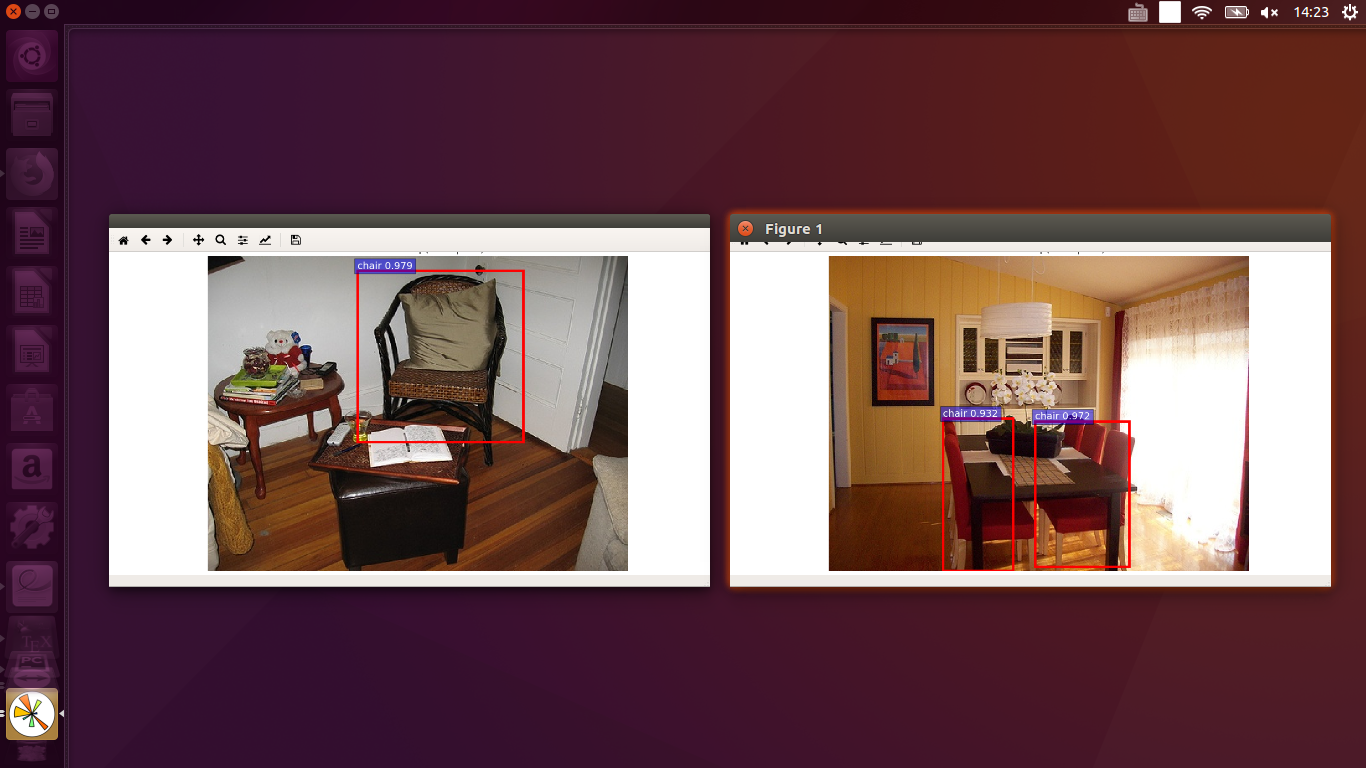
\includegraphics[scale=0.15]{figures/18.png} 
	} 
	\subfigure[Model files]{ 
		\label{p17b} %% label for second subfigure 
		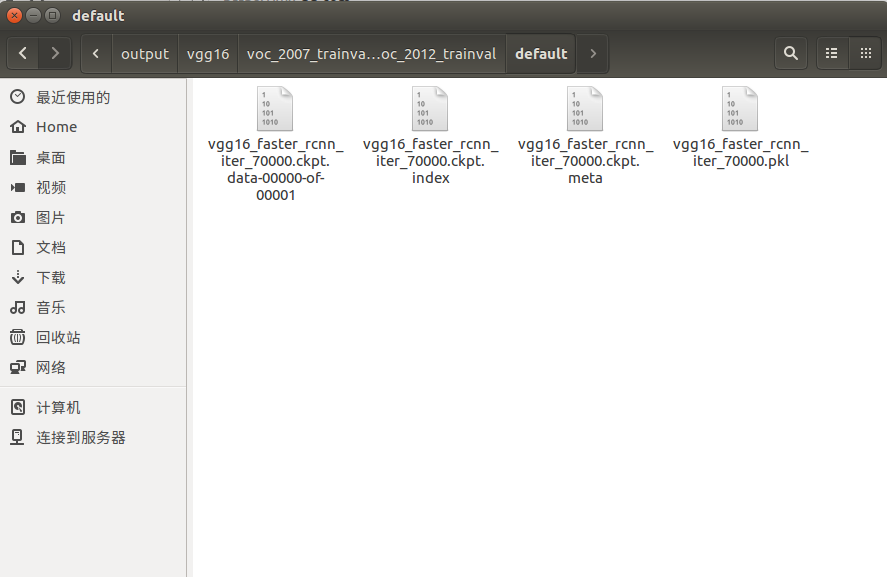
\includegraphics[scale=0.19]{figures/19.png} 
	} 
	\caption{Training model and test results} 
	\label{p17} %% label for entire figure 
\end{figure}

\subsection{Deep L-layer neural network}

\begin{figure}
	\begin{center}
		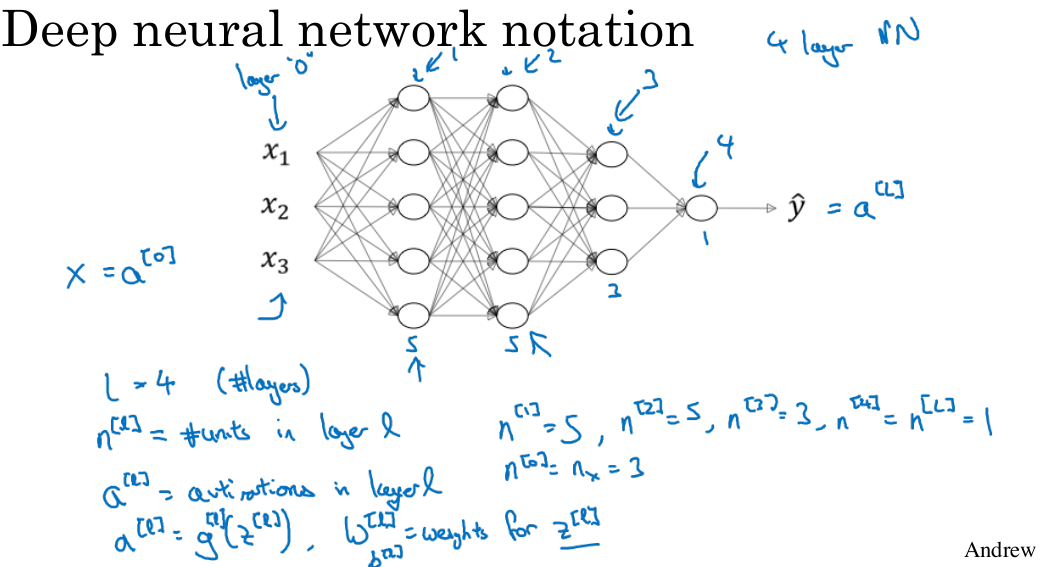
\includegraphics[scale=0.3]{figures/1.png}
	\end{center}
	\caption{Notation in deep neural network in which has four layers with three hidden layers totally.}
	\label{p1}
\end{figure}

In this secton, I go through the notation used to describe deep neural networks first. There is a four-layer neural network with three hidden layers as shown in Fig.~\ref{p1}, in which number of units in hidden layers are five, five and three. So we use L to denote the number of layers in the nerwork and $L = 4$ in this example. Besides, I use $n^{[l]}$ to denote the number of nodes or units in layer and $n^{[i]} = 5$ is the first hidden layer because we have 5 hidden units. So I can get that $n^{[4]} = n^{[l]} = 1$ which is the number of output units. The input layer is $n^{[0]} = n_x = 3$. 
\begin{figure}
	\begin{center}
		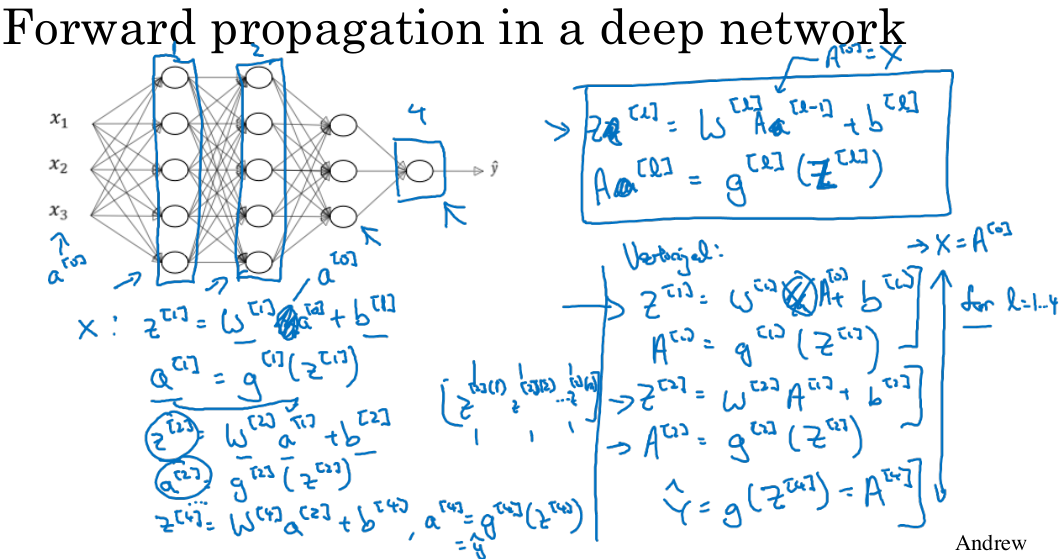
\includegraphics[scale=0.3]{figures/2.png}
	\end{center}
	\caption{Forward propagation in a deep network.}
	\label{p2}
\end{figure}

For each layer, we use $n^{[l]}$ to denote the activations in layer l and $w^{[l]}$ to compute the values $Z^{[l]}$ in the $a^{[l]}$ similatly the $b^{[l]}$ is. In summary, the input features are called x, which is alse the activstion of layer 0 that is $a^{[0]}$ as well and the activation of the final layer $a^{[L]} = \hat{y}$ which also means predicted output.


\subsection{Forward and Backward Propagation}

Then I learn how to perform for propagation in a deep network. As shown in Fig.~\ref{p2}, we can know the process and vectorized version on the left of diagram. $W^{[1]}$, which is a weight matrix, and $b^{[1]}$, which is the bias vector, are parameters affect the activations in layer 1 of the neural network. The activation function g depends on the layer. Besides, we can change x into $a^{[0]}$. And the general rule is that $Z^{[1]} = W^{[1]}\times A^{[l-1]}+b^{[l]}$ and $A^{[1]} = g^{[1]}(Z^{[1]})$ as shown in left diagram below, which gives the vectorized version of forward propagation. As we can see, the implementation of vectorization like a for loop, that is from 1 through the total number of layers and in neural network is perfectly okay to have an explicit for loop.
\begin{figure}
	\centering 
	\subfigure[]{ 
		\label{p3a} %% label for first subfigure 
		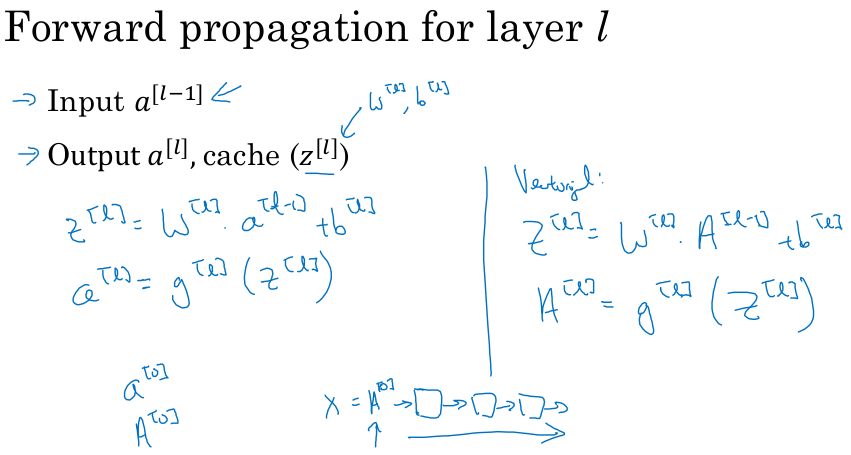
\includegraphics[scale=0.2]{figures/3.png} 
	} 
	\subfigure[]{ 
		\label{p3b} %% label for second subfigure 
		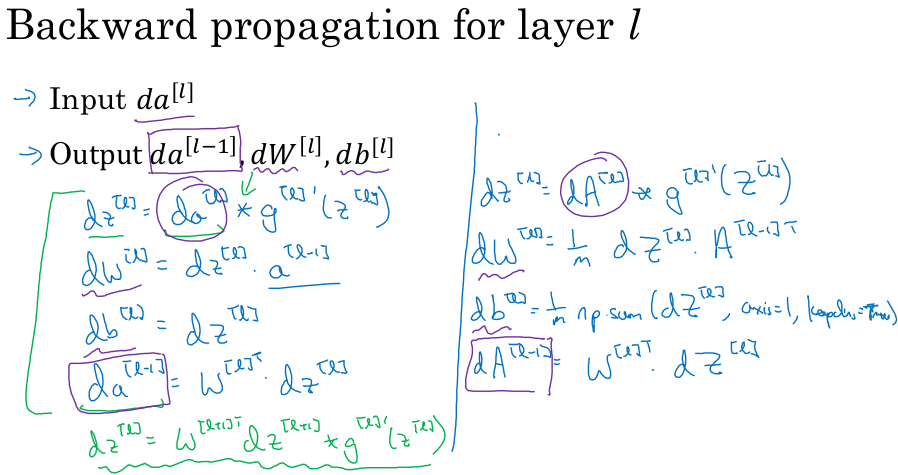
\includegraphics[scale=0.2]{figures/4.png} 
	} 
	\caption{Forward and backward propagation} 
	\label{p3} %% label for entire figure 
\end{figure} 


Then I know how to implement forward and backward propagation steps with basic blocks of a deep neural network in Fig.~\ref{p3}. The way to improve the forward funciton is $Z^{[l]}=W^{[l]}\times a^{[l-1]}+b^{[l]}$ and $a^{[l]}=g^{[l]}\times (Z^{[l]})$ which can be a vectorized implementation $Z^{[l]}=W^{[l]}\times A^{[l-1]}+b^{[l]}$ and $A^{[l]}=g^{[l]}\times (Z^{[l]})$ where the b being python broadcasting just as shown in Fig.~\ref{p3}\subref{p3a}. If we are processing the entire training set, $A^{[0]}$ is the entire training. So it is the input to the first forward function in the chain.

However, the backward propagation steps is shown in Fig.~\ref{p3}\subref{p3b}, which are $dZ^{[l]}=da^{[l]}\times g^{[l]\prime}\times (Z^{[l]})$, $dW^{[l]}=dZ^{[l]}$ and etc. In summary as Fig.~\ref{p4}, we may have the first and second layer maybe has a ReLU activation function but sigmoid activation function in the third layer and the output is $\hat{y}$ if we are doing binary classification. And then using $\hat{y}$ can compute the loss, this allows we to start backward iteration as backward propagation to compute the derivatives. We should know that $da^{[l]}=-\frac{y}{a}+\frac{1-y}{1-a}$ which turns out that the derivative of the loss function respect to the output.

\begin{figure}[!b]
	\begin{center}
		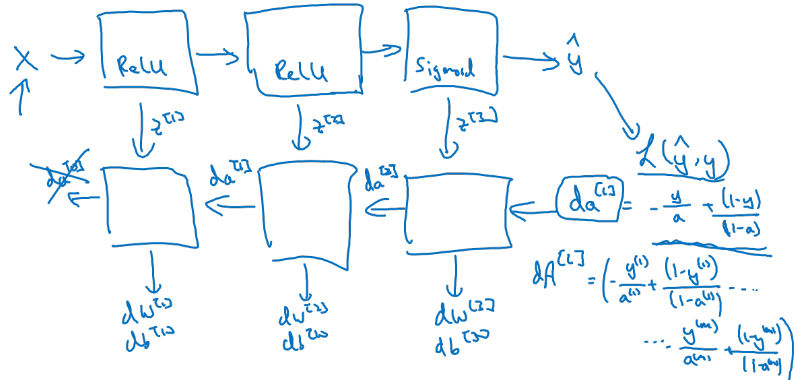
\includegraphics[scale=0.3]{figures/5.png}
	\end{center}
	\caption{Building blocks of deep neural networks.}
	\label{p4}
\end{figure}

\subsection{Intuition about Deep Representation}
If we are building a system for face recogniton or detection as shown in Fig.~\ref{p5}. Perhaps we input a picture of a face then the first layer of the neural network you can think of as maybe being a feature detector or an edge detector. In this example, we're plotting what a neural network with maybe 20 hidden units, might be kind of compute on this image. So the 20 hidden units visualize by these little square boxes. For example, this little visualization represents a hidden unit is trying to figure out if where the edges of that orientation in DMH. And maybe this hidden unit maybe trying to figure out where are the horizontal edges in this image.  Now we think about where the edges in this picture by grouping together pixels to form edges. It can then detect the edges and group edges together to form parts of faces.
\begin{figure}
	\begin{center}
		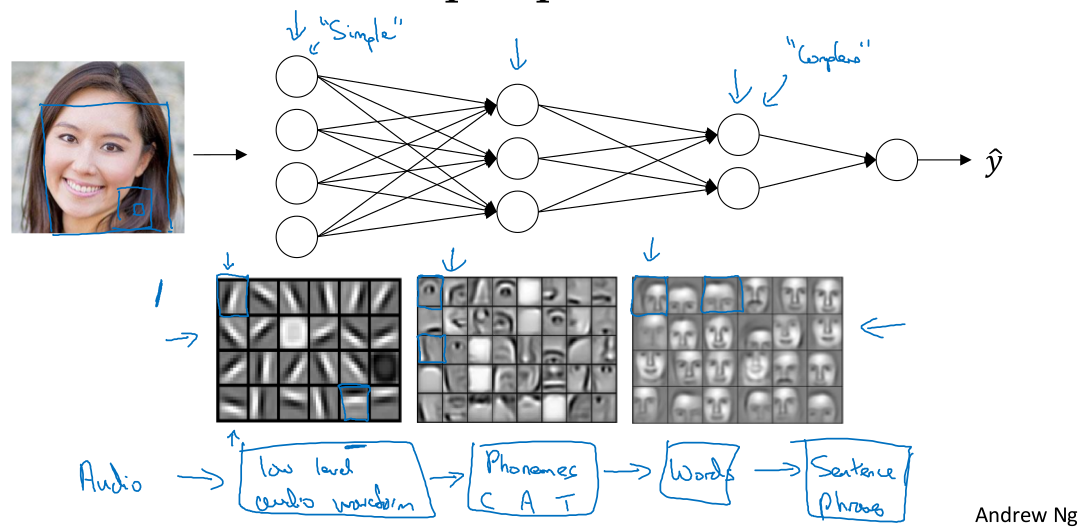
\includegraphics[scale=0.3]{figures/6.png}
	\end{center}
	\caption{Face recogniton.}
	\label{p5}
\end{figure}

\subsection{Train / Dev / Test sets}

From this section, I learn the practical aspects to make neural network work well, ranging from things like hyperparameter tuning to how to set up data and make sure optimization algorithm runs quickly, in order to get our learning algorithm to learn in a reasonable time.

Making good choices in how to set up training, development and test sets can make a huge different in helping us quickly find a good high performance neural network. So in practice applied machine learning is a highly iterative process. Even very experienced deep learning people find it almost impossible to correctly, and then applied deep leanring is a very iterative process where we just have to go around this cycle many times to hoprfully find a good choice of network for application. 

Training data is carve off some portion of it to be training set. And some portion of it to be hold-out cross validation set which sometimes also called development set. Then some final portion of it to be test set as shown in Fig.~\ref{p6}. In order to get an unbiased estimate of how well algorithm is doing, it was common practice to take all data and split it according to maybe a 70/30\% in terms of people often talk about 70\% train and 30\% test splits or maybe a 60\% train, 20\% dev, and 20\% test which is widely considered best practice in machine learning. However, we also seen applications where if we have even more than a million examples, we might with 99.5\% train, 0.25\% and 0.25\% test. Besides, the development and test sets should come from the same distribution. Furthermore, having set up a train dev and test set will allow to integrate more quickly, which allow to more efficiently measure the bias and variance of the algorithm.
\begin{figure}
	\begin{center}
		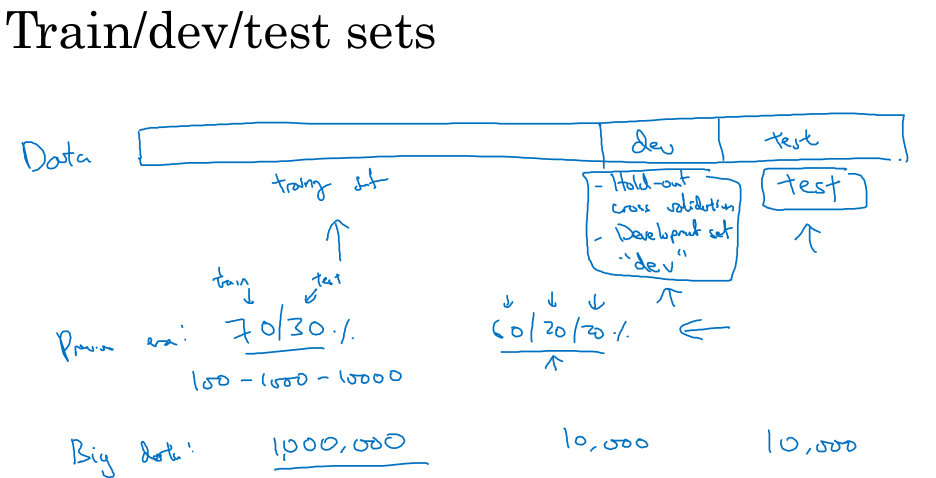
\includegraphics[scale=0.3]{figures/7.png}
	\end{center}
	\caption{Train / Dev / Test sets.}
	\label{p6}
\end{figure}

\subsection{Bias and Variance}

Bias and Variance is one of those concepts that is easily learned but difficult to master. We see the data set that looks like this in Fig.~\ref{p7}. From class of a high bias, if we fit a straight line to the data, maybe get a logistic regression but is not a very good fit to the data, what we say that is underfitting the data. On the oppsite end, if we fit an incredibly complex classifier, here is a classifier of high variance and is overfitting the data. And there might be some classifier in between, with a medium level of complexity and fits it correctly, so we call that just right, it is somewhere in between.
\begin{figure}
	\begin{center}
		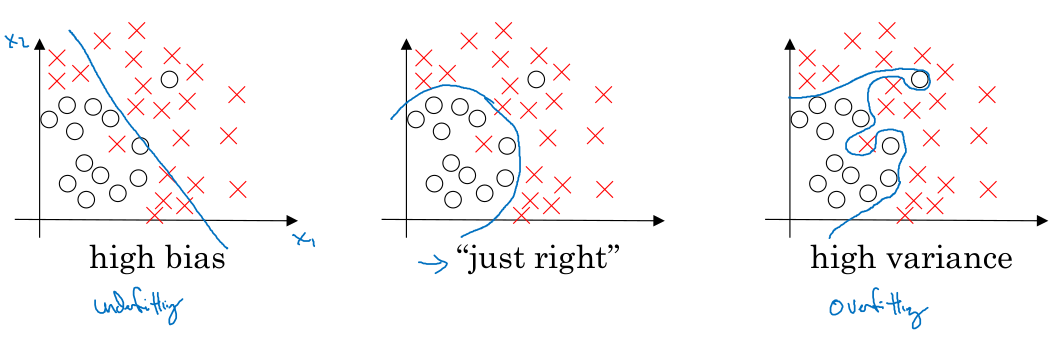
\includegraphics[scale=0.3]{figures/8.png}
	\end{center}
	\caption{Bias and variance.}
	\label{p7}
\end{figure}

More generally, the optimal error called Bayes error. So the case of how to analyze bias and variance, the takeway is that by looking at your training set error. We can get a sense of how well you are fitting and looking at how much higher error goes. When you go from the training set to the dev set, that should give us a sense of how bad is the variance problem. Training and depth error can help us wether algorithm has a bias or variance problem or maybe both, which turns out that this information lets us much more systematically using what they call a basic recipe for machine learning.

When training a neural network, here a basic recipe in Fig.~\ref{p8}. After training a initial model, we should know how algorithm is high or not and so to try and evaluate if there is high bias. Besides, the training set or data performance. If it has  high bias, even does not fit in the training set, we could try pick a network such as more hidden layers or more hidden units. 
\begin{figure}
	\begin{center}
		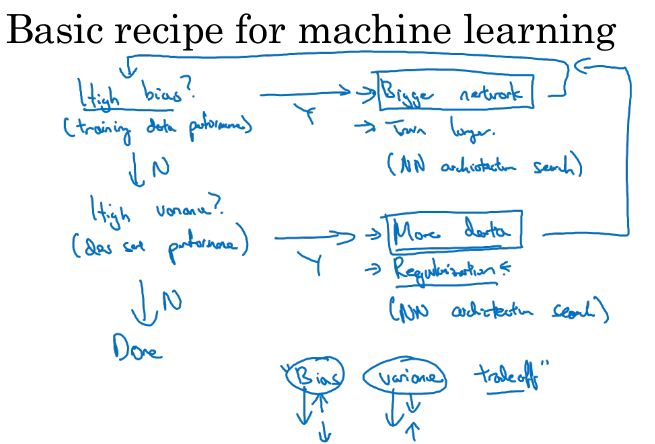
\includegraphics[scale=0.3]{figures/9.png}
	\end{center}
	\caption{Basic recipe for machine learning.}
	\label{p8}
\end{figure}

So when training a learning algorithm, we should try these things until at least get rid of the bias problem or fit the training set pretty well. And so to evaluate variance, we would look at dev set performance. If if it is high, the best way to solve a high variance problem is to ger more data. However, when we cannot get more, we could try regularization to reduce overfitting. So being clear on how much of a bias or variance problem or both can help us focus on selecting the most useful things to try.

\subsection{Regularization Reduces Overfitting}
If we suspect  neural network is overfitting your data, one of the first things we should try is probably regularization. But adding it will often help to prevent overfitting. The other way to address high variance is to get more training data which is alse quite reliable. We develop these prevent ideas using logistic regression. And so to add regularization to the logistic regression, what you do is add to it like $J(w,b)=\frac{1}{m}\sum_{i=1}^{m}\mathcal{L}(\hat{y}^{(i)},y^{(i)})+\frac{\lambda}{2m}\parallel w\parallel^2_2$ where $\lambda$ is the rregularization parameter and $\parallel w\parallel^2_2$ is norm of w squared is a square Euclidean norm of the parameter vector w as shown in Fig.~\ref{p9}, which is called L2 regularization. Because w is usually a high dimensional parameter vector, especially with a high variance problem, we just omit b. In a word, L2 regularization is the most common type of regularization which is called weight decay as well. We can also call it Frobenius norm of the matrix as $\parallel w^{[l]}\parallel^2_F=\sum_{i=1}^{n^{[l-1]}}\sum_{j=1}^{n^{[l]}}(w_{ij}^{[l]})^2$.
\begin{figure}
	\begin{center}
		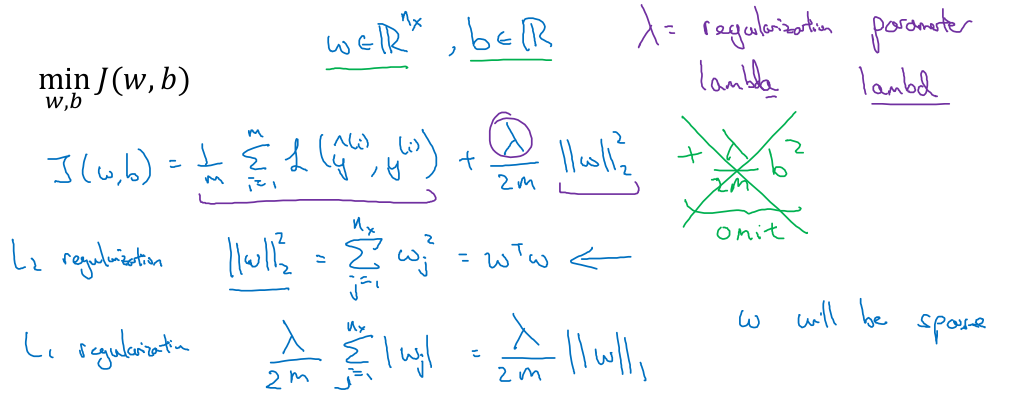
\includegraphics[scale=0.3]{figures/10.png}
	\end{center}
	\caption{Logistic regression.}
	\label{p9}
\end{figure}

We can know the reason why regularization help with overfitting from a couple example in Fig.~\ref{p10}. The cost function $J(w^{[l]},b)=\frac{1}{m}\sum_{i=1}^{m}\mathcal{L}(\hat{y}^{(i)},y^{(i)})+\frac{\lambda}{2m}\parallel w\parallel^2_2$ which can penalize the weight matrices from being too large. The Frobenius morm might cause less overfiting because of one piece of intuition is that if you crank regularisation lambda to be really big, they will be incentivized to set the weigth matrices W to be reasonably close to zero that is setting the weight to be so close to zero for a lot of hidden units, which basically zeroing out a lot of the impact of these hidden units. If implementing regularization, we should remember J now has a new definition above. The new funciton is to debug gradient descent otherwise might not see J decrease monotonically on every single elevation. 
\begin{figure}
	\begin{center}
		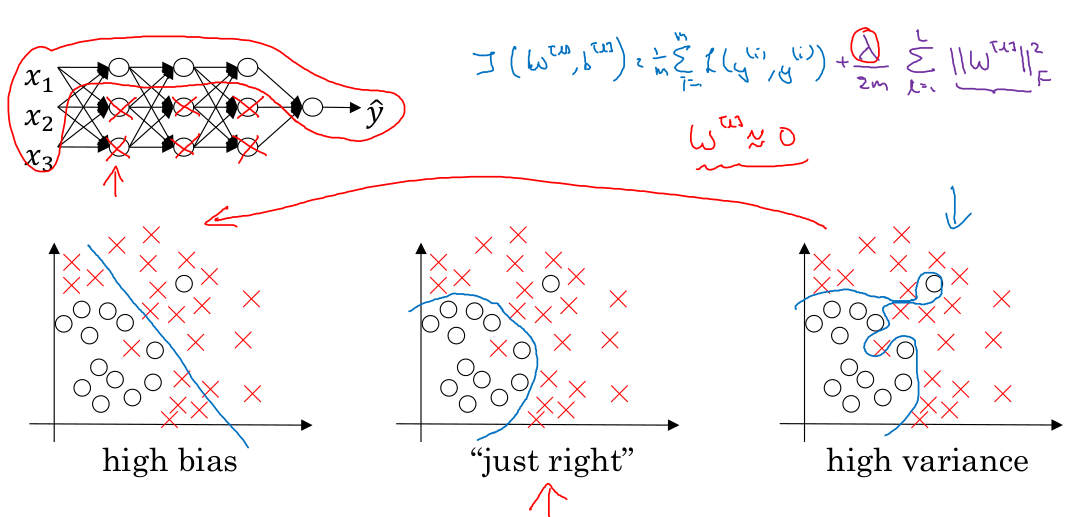
\includegraphics[scale=0.3]{figures/11.png}
	\end{center}
	\caption{Examples of regularization help with overfitting.}
	\label{p10}
\end{figure}

In addition to L2 regularization, there is another powerful regularization techniques which is called dropout. With dropout, what we are going to do is to go through each of the layers of the network and set some probability of eliminating a node in neural network as shown in Fig.~\ref{p11}. So we end up with a much smaller, really much diminished network and then do back propagation training. Inverted dropout is one of ways of implementing dropout but if we are implementing dropout at test time, that just add noise to predictions. By spreading all the weights, this will tend to have an effect of shrinking the squared norm of the weights, and so, similiar to what we saw with L2 regularization, the effect of implementing dropout is that it shrinks the weights and does some of those outer regularization that helps prevent overfitting. 
\begin{figure}
	\begin{center}
		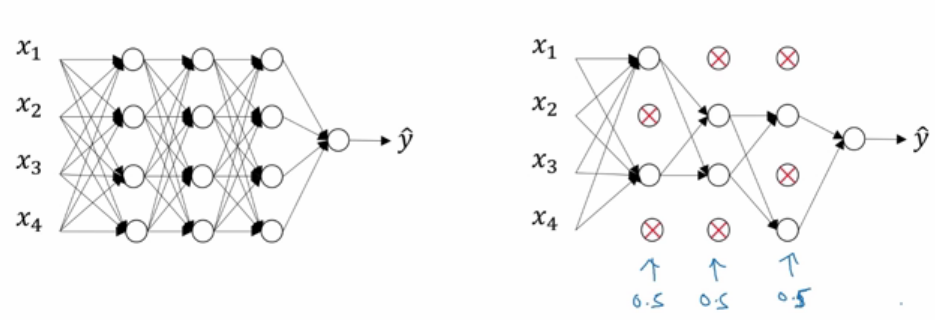
\includegraphics[scale=0.3]{figures/12.png}
	\end{center}
	\caption{Dropout regularization technique.}
	\label{p11}
\end{figure}
These could be different keep probs for different layers. Notice that the keep prob of one means that we are keeping every units. However, for layers where we are more worried about ever-fitting and layers with lots of parameters, we can set keep prob to be smaller to apply a more powerful form of dropout. If we are more worried about some layers overfitting than others, we can set lower keep prob for some layers than others. So in computer vision, the input size is so big, putting all these pixels that you almost never have enough data, so dropout is very frequently used by computer vision. However, ont big downside of dropout is that the cost function J is no longer well-defined. On every iteration, we are randomly killing off a bunch of nodes.

There are a few other techniques for reducing overfitting in your neural network, in addition to L2 regularization and dropout. If we are fitting a cat classifier, we can augment training set by taking image like flipping it horizontally or rotate. And double the size of training set. We can do this without needing to pay the expense of going out to take more pictures of cats as fake training examples. 

When training a neural network, one of the techniques that will speed up our training is normalize inputs which corresponds to two steps as shown in Fig.~\ref{p12}. The first is to subtract out or to zero out the mean. And then the second step is to normalize the variances, which X1 and X2 are both equal to one. We use this to scale train data, then should use the same $\mu$ and $\sigma^2$ to normalize test set other than estimate $\mu$ and $\sigma^2$ separately on your training and test set. Because we want our data, both training and test examples to go through the same transformation defined by the same $\mu$ and $\sigma^2$. If input features came from very different scales then it is important to normalize your features.
\begin{figure}
	\begin{center}
		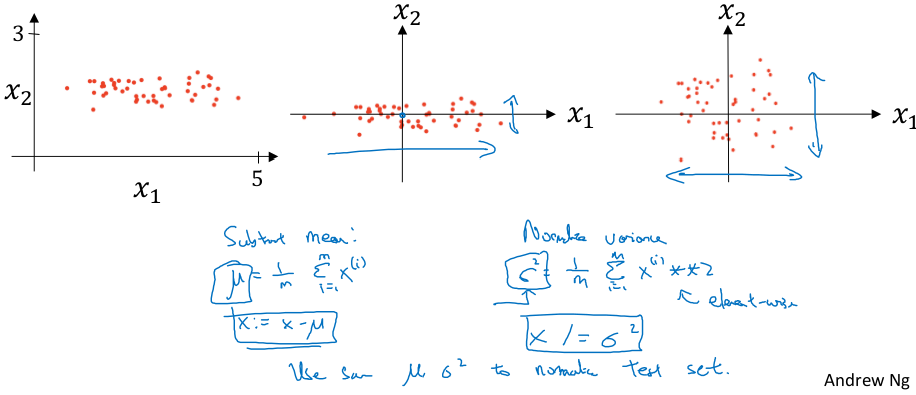
\includegraphics[scale=0.3]{figures/13.png}
	\end{center}
	\caption{Normalizing training sets.}
	\label{p12}
\end{figure}

\subsection{Gradient Checking}
One of the problems of training neural network, especially very deep neural network is data vanishing or exploding gradients. At the weights W, if they are all just a little bit bigger than 1 or identity matrix, then with a very deep network, the activations can explode. In contrast, if W is just a little bit less than identity, so the activations will decrease exponentially.

To prevent vanishing or exploding, we start with the example of initializing the weights for a single neuron in Fig.~\ref{p13}. In order to make z not blow up and become too small. One reasonable thing to do would be set the variance of $W^{[i]}=\frac{1}{n}$. So in practice, what you can do is set the weight matrix W for a certain layer $W^{[l]}=np.random.randn(shape)\times np.sqrt(\frac{1}{n^{[l-1]}})$ because that is the number of units that we are fitting in to each of the units of layer l. And it definitely helps reduce the vanishing, exploding gradients problem because it is trying to set each of the weight matrices w.
\begin{figure}
	\begin{center}
		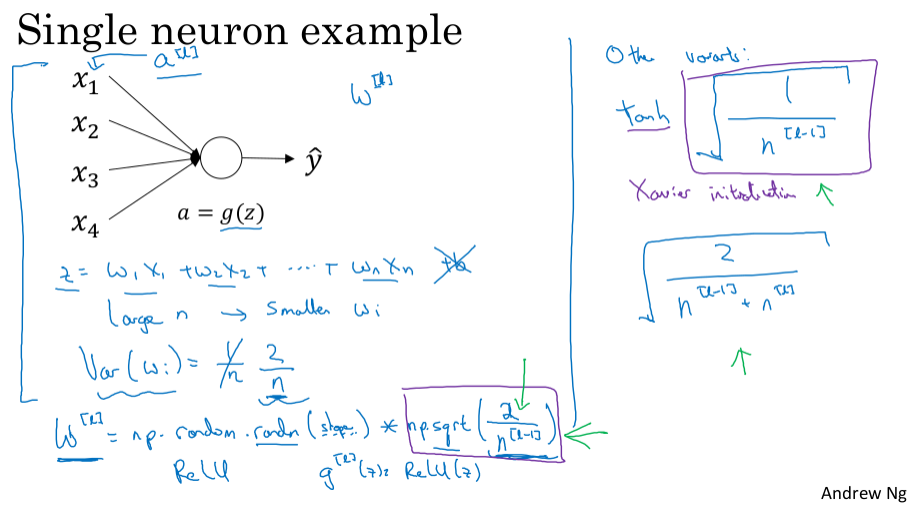
\includegraphics[scale=0.3]{figures/14.png}
	\end{center}
	\caption{Single neuron example.}
	\label{p13}
\end{figure}

When implement back propagation, we will find that there's a test called creating checking that can really help make sure that implementation of back prop is correct. The first stage is to numerically approximate computations of gradients in Fig.~\ref{p14} from which demonstrates two sided difference way of approximating the derivative is extremely close to 3. And so this gives you a much greater confidence that $g(\theta)$ is a correct implementation of the derivative of f. So when doing gradient checking, we rather use this two-sided difference when you compute $g(\theta)=\frac{f(\theta+\epsilon)-f(\theta-\epsilon)}{2\epsilon}$. And the takeway is that this teo-sided difference formula is much more accurate.
\begin{figure}
	\begin{center}
		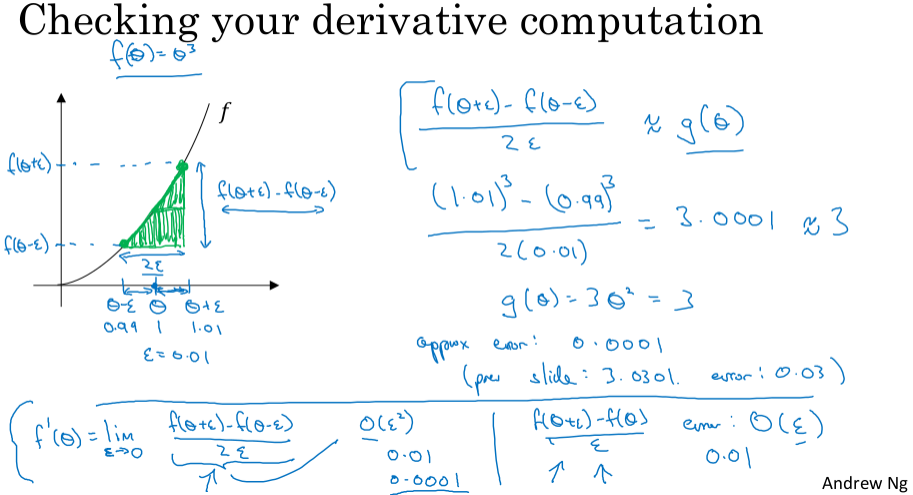
\includegraphics[scale=0.3]{figures/15.png}
	\end{center}
	\caption{Checking derivative computation.}
	\label{p14}
\end{figure}

Then we should know that function J is a giant parameter. Whatever's the dimension of this giant parameter vector $\theta$. So to implement grad check, what we are going to do is implements a loop just as equations $d\theta_{appear}[i]\approx \frac{\partial J}{\partial \theta_i}$ in Fig.~\ref{p15}.  
\begin{figure}
	\begin{center}
		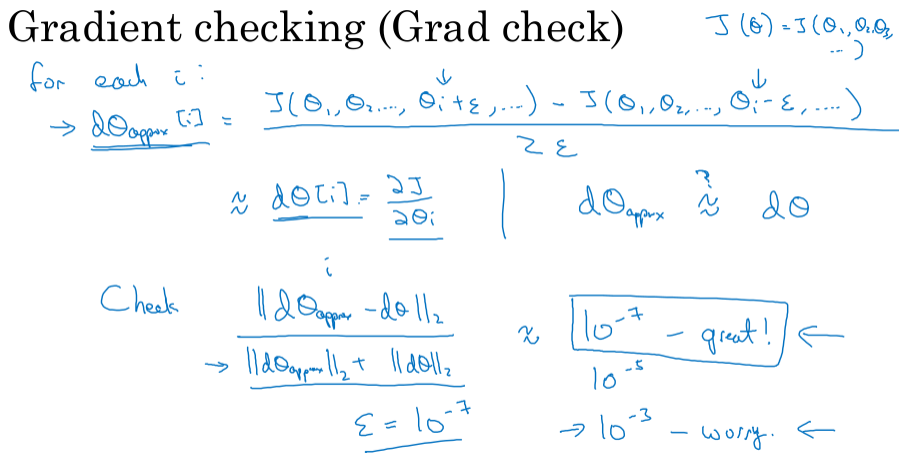
\includegraphics[scale=0.3]{figures/16.png}
	\end{center}
	\caption{Checking derivative computation.}
	\label{p15}
\end{figure}
Then check $\parallel d\theta_{appear}-d\theta \parallel_2$ with no square on top which si Euclidean distance and then to normalize by the lengths of these vectors. So we implement this in practice, $\epsilon$ maybe $10^{-7}$ then value of formular equals to $10^{-7}$ or smaller, then that's great. We use it to track down whether or not some of your derivative computations might be incorrect. And after some amounts of debugging, it finally ends up being a very small value which turns out a correct implementation. When inplement neural network, we often implement foreprop and backprop and debug for a while, we find if passes grad check with a small value. Note that, grad check is used to debug rather than train.

\subsection{Mini-batch Gradient Descent}
Optimizating algorithms helps to train models quickly because training on a large data set is just slow. From courses before, I can know that vectorization allows to process all examples relatively fast but if they are very large then it can still be slow. What we should do is to split up training set into smaller and little baby training sets which are called mini-batches. Batch gradient descent refers to viewing that as processing entire batch of training samples all ai the same time and which we orocess is single mini batch rather than processing entire train set the same time. We get a new notation $X^{\{t\}}$ as shown in Fig.~\ref{p16}. If we have 5 million train samples total, each of these little mini batches has a thousand examples, we would have 5000 of these mini batches, so it ends with $X^{\{5000\}}$ and similarly to Y. Mini batch number t is comprised of $X^{\{t\}}$ and $Y^{\{t\}}$ that is a thousand samples with the corresponding input and output pairs. In summary, $X^{(i)}$ is the i training sample, [l] of $X^{[l]}$ is to index the different layers of the neural network. 
\begin{figure}
	\begin{center}
		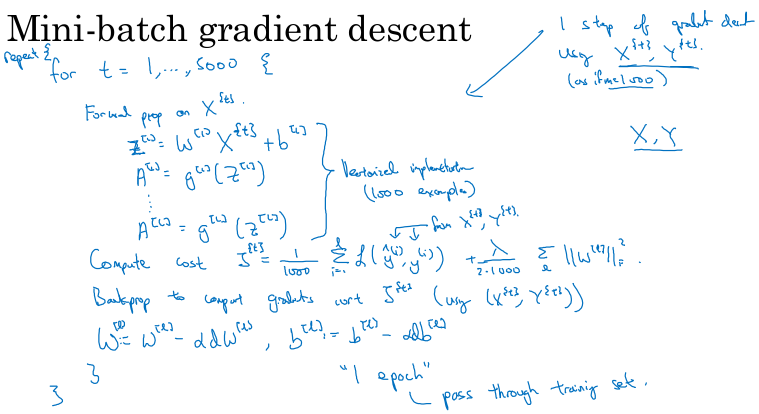
\includegraphics[scale=0.5]{figures/17.png}
	\end{center}
	\caption{Mini-batch gradient descent.}
	\label{p16}
\end{figure}

The process is one pass through training set using mini-batch gradient descent. The code is also called doing one epoch of training and epoch is a word that means a single pass through the train set. With mini-batch gradient descent, a single pass through the training set, allows to take 5000 gradient descent steps.

On mini batch gradient descent though, if plot progress on cost function, it may not decrease on every iteration. In particular, on every iteration we are processing some $X^{\{t\}}$ and $Y^{\{t\}}$. If we plot the cost funciton $J^{\{t\}}$, we more likely to see lines trend downwards but is going to be a little bit noisier.



\section{Progress in this week}

This week for deep learning course of Anandrew Ng, I know about how to set up train, dev and test sets. Besides, I can try to analyze bias and variance and know what things to do if we may have high bias and variance versus. Furthermore, I also understand how to apply different forms of regularization and dropout on neural network. Some tricks for speeding up the training of neural network as well. Last but not least, I learn a little about gradient checking. As for URPC2018, I learn to train the first model with standard VOC2007 data set and test it with photos. Fortunately, test outcomes with model is good that I achieve a little goal at the present stage as shown in table blow.
\begin{description}
	\item [Step 1] Finish training the first VOC2007 model and getting good outcome.
	\item[Step 2] Finish changing the txt truth table into xml files which are used for training contest model.
	\item[Step 3] Finish putting confusing contest data sets in VOC2007 order.
	\item[Step 4] Finish learning improving deep neural network course which is the second lesson.\label{t1}
\end{description}

\section{Plan}

\begin{tabular}{rl}
	\textbf{Objective:} & Finish training a model with contest data sets for URPC2018 \\
	\textbf{Deadline:} & 2018.07.24
\end{tabular}

\begin{description}
	\item[\normalfont 2018.07.16---2018.07.22] Finish neural networks and Deep Learning.
	\item[\normalfont 2018.07.23---2018.07.29] Finish improving deep neural networks courses.
	\item[\normalfont 2018.07.30---2018.08.05] Finish structuring machine learning projects courses.
	\item[\normalfont 2018.08.06---2018.08.12] Finish convolutional neural networks courses.
	\item[\normalfont 2018.08.13---2018.08.19] Finish sequence models courses.
\end{description}



% If you don't cite any references, please comment the following two lines
\bibliographystyle{ieee}
\bibliography{ref.bib}

\end{document}